

\documentclass{beamer}



\mode<presentation>
{
  \usetheme{Frankfurt}
  % or ...

  %\setbeamercovered{transparent}
  % or whatever (possibly just delete it)
}
\usepackage[slovene]{babel}
\usepackage[utf8]{inputenc}
%\usepackage[pdftex]{graphicx}
%\usepackage{color}
%\usepackage{float}
%\usepackage{eurosym}

\usepackage{amsfonts}
\usepackage{amsmath,amsthm}

%\usepackage[english]{babel}
% or whatever

%\usepackage[latin1]{inputenc}
% or whatever

%\usepackage{beamerthemeshadow}
\usepackage{times}
%\usepackage[T1]{fontenc}
% Or whatever. Note that the encoding and the font should match. If T1
% does not look nice, try deleting the line with the fontenc.

\newcommand{\bx}{\mathbf{x}}
\DeclareMathOperator{\Gl}{Gl}
\DeclareMathOperator{\adj}{adj}
%\newcommand{\Gl}{{\mathrm {GL}}\,}
%\newizrek{proposition}[izrek]{Proposition}

% finan�ni instrumenti
\newcommand{\PV}{\mathrm{PV}}


\newcommand{\ds}{\displaystyle}
\newcommand{\ts}{\textstyle}
\newcommand{\presledek}{\vspace{3mm}}
\newcommand{\ph}{\phantom{1}} % pomoč pri poravnavi teksta v slikah TikZ


\newcommand{\abs}[1]{ \left\lvert#1\right\rvert} 
\newcommand{\norm}[1]{\left\lVert#1\right\rVert}
\newcommand{\Co}{\operatorname{Co}} %konveksna ogrinjača

\newcommand{\R}{\mathbb R}
\newcommand{\N}{\mathbb N}
\newcommand{\Z}{\mathbb Z}
\newcommand{\C}{\mathbb C}
\newcommand{\Q}{\mathbb Q}
\newtheorem{izrek}{Izrek}
\newtheorem{lema}[izrek]{Lema}
\newtheorem{trditev}[izrek]{Trditev}
\newtheorem{posledica}[izrek]{Posledica}
\newtheorem{definicija}[izrek]{Definicija}
\newtheorem{naloga}[izrek]{Naloga}
\newtheorem{resitev}[izrek]{Naloga}
\setbeamertemplate{lema}[numbered]


\title[Računanje izotropnih vektorjev] % (optional, use only with long paper titles)
{Računanje izotropnih vektorjev}

%\subtitle
%{Presentation Subtitle} % (optional)

\author[Mirjam Pergar] % (optional, use only with lots of authors)
{\textbf{Avtor:}  Mirjam Pergar\\
\textbf{Mentor:} izred. prof. dr. Bor Plestenjak
}
% - Use the \inst{?} command only if the authors have different
%   affiliation.

\institute[Fakuleta za matematiko in fiziko] % (optional, but mostly needed)
{
%  \inst{1}%

%  \and
%  \inst{2}%
%  Department of Theoretical Philosophy\\
%  University of Elsewhere
}
% - Use the \inst command only if there are several affiliations.
% - Keep it simple, no one is interested in your street address.

\date[24. november 2015] % (optional)
{24. november 2015}

\subject{Talks}
% This is only inserted into the PDF information catalog. Can be left
% out.



% If you have a file called "university-logo-filename.xxx", where xxx
% is a graphic format that can be processed by latex or pdflatex,
% resp., then you can add a logo as follows:

% \pgfdeclareimage[height=0.5cm]{university-logo}{university-logo-filename}
% \logo{\pgfuseimage{university-logo}}



% Delete this, if you do not want the table of contents to pop up at
% the beginning of each subsection:
%\AtBeginSubsection[]
%{
%  \begin{frame}<beamer>
%    \frametitle{Outline}
%    \tableofcontents[currentsection,currentsubsection]
%  \end{frame}
%}


% If you wish to uncover everything in a step-wise fashion, uncomment
% the following command:

%\beamerdefaultoverlayspecification{<+->}
\setbeamertemplate{footline}[frame number]

\begin{document}

\begin{frame}
  \titlepage
\end{frame}

\begin{frame}
  \frametitle{Vsebina}
  \tableofcontents[pausesections]
  % You might wish to add the option [pausesections]
\end{frame}


\section{Uvod}
\subsection{Problem}
\begin{frame}
  \frametitle{Problem}
\begin{alertblock}{}
Za dano nesingularno, kvadratno $n \times n$ matriko $A$ z realnimi ali kompleksnimi elementi, nas zanima izračun enotskega vektorja $b$ z realnimi ali kompleksnimi elementi, tako da velja:
\begin{equation}\label{eq:zac}
b^\ast Ab=0.
\end{equation}
Vektor $b$, za katerega velja \eqref{eq:zac} in $b^\ast b=1$  imenujemo \textbf{izotropni vektor}. 
Bolj splošen je inverzni problem zaloge vrednosti, kjer iščemo enotski vektor $b$, za katerega velja:
\begin{equation}\label{eq:splosno}
b^\ast Ab=\mu,
\end{equation}
kjer je $\mu$ dano kompleksno število.
\end{alertblock}
\end{frame}
\begin{frame}
\begin{itemize}
\item Problem \eqref{eq:splosno} je možno prevesti na problem \eqref{eq:zac} za drugo matriko, saj je \eqref{eq:splosno} enako
$$b^\ast (A-\mu I)b=0.$$
\item Če $\mu$ lastna vrednost matrike $A$, potem je rešitev pripadajoč lastni vektor matrike $A$.
\item Če $\mu$ ni lastna vrednost matrike $A$, je $A-\mu I$ nesingularna in je potreben izračun izotropnega vektorja te matrike.
\item Od sedaj naprej bomo vse vrednosti enačili z $0$.
\end{itemize}
\end{frame}
\begin{frame}
\frametitle{Zaloga vrednosti}
\begin{definicija}
\textbf{Zaloga vrednosti} matrike $A \in \C^{n\times n}$ je podmnožica kompleksne ravnine, definirana kot
$$W(A)=\{x^\ast Ax: x \in \C^n, x^\ast x=1\}.$$
\end{definicija}\pause
\begin{itemize}
\item Očitno je $W(A)$ množica vseh Rayleighovih kvocientov matrike $A$.
\item Izhodišče mora biti v $W(A)$, če hočemo, da ima \eqref{eq:zac} vsaj eno rešitev.
\item Označimo s $\sigma(A)$ množico vseh lastnih vrednosti matrike A, ki jo imenujemo spekter.
\end{itemize}
\end{frame}
\begin{frame}
\frametitle{Lastnosti zaloge vrednosti}
\begin{enumerate}
\item $W(A)$ je konveksna, zaprta in omejena.
\item $\sigma(A)\subseteq W(A).$
\item Za vsako unitarno matriko $U$ je $W(U^\ast AU)=W(A).$
\item $W(A+zI)=W(A)+z$ in $W(zA)=zW(A)$ za vsako kompleksno število $z$.
\item Rob zaloge vrednosti $W(A), \partial W(A)$ je kosoma algebrajska krivulja, in vsaka točka v kateri $\partial W(A)$ ni diferenciabilna je lastna vrednost matrike $A$.
\item Če je $A$ normalna, potem $W(A)=\Co(\sigma(A))$, kjer s $\Co$ označimo zaprto konveksno ogrinjačo množice.
\item $W(A)$ je daljica na realni osi, če in samo če je $A$ hermitska.
\end{enumerate}
\end{frame}
\begin{frame}
\begin{izrek}
Naj imata $A$ in $b$ realne ali kompleksne elemente. Potem veljajo enakosti:
$$b^\ast Ab=0\Leftrightarrow b^\ast (A+A^\ast)b=0 \quad \text{in}\quad  b^\ast(A-A^\ast)b=0.$$
\end{izrek}\pause
\begin{proof}
($\Rightarrow$) Če velja $b^\ast Ab=0$, je tudi $(b^\ast Ab)^\ast=b^\ast A^\ast b=0$. Preoblikujemo prvo enačbo na desni v $b^\ast Ab +b^\ast A^\ast b$ dobimo 0. Drugo enačbo dokažemo na podoben način.\\
($\Leftarrow$) S seštevkom enačb na desni dobimo enačbo na levi:
\begin{align*}
 b^\ast (A+A^\ast)b+b^\ast(A-A^\ast)b=0\\
b^\ast (2A)b=0\\
b^\ast Ab=0
\end{align*}
\end{proof}
\end{frame}
\begin{frame}
\begin{itemize}
\item Če velja le $b^\ast (A+A^\ast)b=0 \Rightarrow \Re(b^\ast Ab)=0$.
\item Če velja le $b^\ast(A-A^\ast)b=0 \Rightarrow \Im(b^\ast Ab)=0$.
\item Označimo z $A_{sim}=A^T$ simetrični del matrike $A$ in z $A_{psim}=-A^T$ poševno-simetrični del matrike $A$.
\end{itemize}\pause
\begin{lema} %\cite{lipkin}
Izotropni vektorji matrike A so identični izotropnim vektorjem njenega simetričnega dela.
\end{lema} \pause
\begin{proof}
To sledi iz $b^T Ab=b^T A_{sim} b +b^T A_{psim} b=b^T A_{sim} b,$ kjer je z $A_{sim}$ označen simetrični del matrike $A$  in z $A_{psim}$ poševno-simetrični del matrike A.
\end{proof}
\end{frame}
\begin{frame}
Velja enakost:
\begin{block}{}
$$b^T Ab=0 \Leftrightarrow b^T (A+A^T)b=0.$$ 
\end{block}\pause
\begin{itemize}
\item Hermitski del matrike $A$ bomo označili s $H=(A+A^\ast)/2$.
\item Poševno-hermitski del matrike $A$ bomo označili z $\tilde{K}=(A-A^\ast)/2=\imath K$.
\end{itemize}
\end{frame}
\subsection{Uporaba}
\begin{frame}
\frametitle{Uporaba}
\begin{itemize}
\item Preučevanje konvergence nekaterih iterativnih metod za reševanje linearnih sistemov, npr. GMRES.
\item Aplikacije v numerični analizi, diferencialnih enačbah, teoriji sistemov itd.
\end{itemize}
\end{frame}
\section{Realne matrike} %REALNE MATRIKE
\subsection{Uvod}
\begin{frame}
\frametitle{Realne matrike}
\begin{block}{}
Ko je $A$ realna matrika, nas zanima kako se izračuna rešitev enačbe:
\begin{equation}\label{eq:realna}
b^\ast Hb=0,
\end{equation}
kjer je $H$ realna in simetrična matrika (t.j. $H=H^T$).
\end{block}\pause
Vemo:
\begin{itemize}
\item $W(A)$ simetrična glede na realno os.
\item $0 \in W(A)$, če in samo če $\lambda_n\le0\le\lambda_1$, kjer sta $\lambda_n$ in $\lambda_1$ najmanjša in največja lastna vrednost matrike $H$.
\end{itemize}
\end{frame}
\begin{frame}
Naj bosta $x_1$ in $x_n$ realna lastna vektorja, pripadajoča $\lambda_1$ in $\lambda_n$. Potem sta:
\begin{itemize}
\item $x_1^T Ax_1=x_1^T Hx_1=\lambda_1$.
\item $x_n^T Ax_n=x_n^T Hx_n=\lambda_n$.
\end{itemize}
realni točki na skrajni levi in skrajni desni zaloge vrednosti $W(A)$ na realni osi.
\begin{itemize}\pause
\item Realne rešitve \eqref{eq:realna} izračunamo z uporabo lastnih vektorjev matrike $H$. 
\item Predpostavimo, da iščemo vektorje $b$ z normo 1.
\item $H$ zapišemo kot $$H=X\Lambda X^T,$$ kjer je $\Lambda$ matrika, ki ima na diagonali lastne vrednosti $\lambda_i$, ki so realna števila in $X$ je ortogonalna matrika lastnih vektorjev, tako da $X^T X=I$.
\end{itemize}
\end{frame}
\begin{frame}
\begin{itemize}
\item Uporabimo ta spektralni razcep v \eqref{eq:realna}: $$b^\ast Hb=b^\ast X\Lambda X^T b=0.$$ 
\item  Označimo s $c=X^Tb$ vektor projekcije $b$ na lastne vektorje matrike $H$. 
\end{itemize}\pause
\begin{izrek} \label{izrek2}
Naj bo $b$ rešitev problema \eqref{eq:realna}. Potem vektor $c=X^T b$ s komponentami $c_i$ zadošča naslednjima enačbama:
\begin{align}
\sum_{i=1}^{n} \lambda_i \abs{c_i}^2=0 \label{eq:en1},\\
\sum_{i=1}^{n}\abs{c_i}^2=1. \label{eq:en2}
\end{align}
\end{izrek}
\end{frame}
\begin{frame}
\begin{proof}
Enačbo \eqref{eq:en1}  dokažemo tako, da $c=X^Tb$ oz. $c^\ast =b^\ast X$ vstavimo v \eqref{eq:realna} in dobimo $$b^\ast Hb=b^\ast X\Lambda X^T b= c^\ast \Lambda c=0.$$ Ker je $\Lambda$ diagonalna matrika, lahko $c^\ast \Lambda c$ zapišemo kot vsoto komponent $\bar{c_i}\lambda_i c_i=\lambda_i\abs{c_i}^2$, ko $i=1,2,...n$.
Za enačbo \eqref{eq:en2} vemo, da je $\norm{b}_2=1$. Če normo zapišemo s $c$ dobimo $$\norm{b}_2=\norm{Xc}_2=\norm{c}_2=1,$$ saj je $X$ ortogonalna matrika.
\end{proof}
\end{frame}
\subsection{Iskanje izotropnih vektorjev}
\begin{frame}
\frametitle{Iskanje izotropnih vektorjev}
\begin{block}{}
Če predpostavimo, da nimajo vse lastne vrednosti $H$ enakega predznaka, potem mora za najmanjšo lastno vrednost $\lambda_n$ veljati $\lambda_n <0$. 
 Naj bo $k<n$ tak, da je $\lambda_k >0$ in $0<t<1, t\in \R$ .  Označimo $\abs{c_n}^2 =t$,$\abs{c_k}^2=1-t$ in $c_i=0, i\not=n,k$, kar velja zaradi enačbe \eqref{eq:en2}, $t+ (1-t)=1$. Iz \eqref{eq:en1} mora veljati enačba: $$\lambda_n t +\lambda_k (1-t)=0,$$ katere rešitev je:
\begin{equation}
t_s=\frac{\lambda_k}{\lambda_k -\lambda_n}.
\end{equation}
\end{block}
\end{frame}
\begin{frame}
\begin{itemize}
\item Absolutna vrednost $c_n$ (oz. $c_k$) je kvadratni koren od $t_s$ (oz. $1-t_s$).
\item Ker je $b=Xc$, sta dve realni rešitvi: $$b_1=\sqrt{t_s}x_n +\sqrt{1-t_s}x_k,\quad b_2=-\sqrt{t_s}x_n+\sqrt{1-t_s}x_k,$$ kjer sta $x_n$ in $x_k$ lastna vektorja pripadajoča  $\lambda_n$ in $\lambda_k$.\pause
\item Ker imata izraza v rešitvah enaka imenovalca, lahko rešitvi zapišemo kot: $$b_1=\sqrt{\lambda_k}x_n+\sqrt{\abs{\lambda_n}}x_k, \quad b_2=-\sqrt{\lambda_k}x_n+\sqrt{\abs{\lambda_n}}x_k$$.\pause
%(sledi iz \cite{lipkin}).
\item Vektor mora biti normiran:
\begin{align*}
b_1=\sqrt{\frac{\lambda_k}{\lambda_k +\abs{\lambda_n}}}x_n + \sqrt{\frac{\abs{\lambda_n}}{\lambda_k +\abs{\lambda_n}}}x_k,\\ b_2=-\sqrt{\frac{\lambda_k}{\lambda_k +\abs{\lambda_n}}}x_n + \sqrt{\frac{\abs{\lambda_n}}{\lambda_k +\abs{\lambda_n}}}x_k.
\end{align*}
\end{itemize}
\end{frame}
\begin{frame}
\frametitle{Število rešitev}
Uporabimo lahko vsak par pozitivnih in negativnih lastnih vrednosti. Ta postopek lahko vrne toliko rešitev kot je dvakratno število parov lastnih vrednosti matrike $H$ z nasprotnimi predznaki, če so vse lastne vrednosti različne. Predpostavimo, da je $b$ realen.\pause
\begin{posledica}%\cite{lipkin}
Dobljena izotropna vektorja sta ortogonalna ($b_1 ^T b_2=0$), če in samo če $\lambda_k=-\lambda_n$.
\end{posledica}\pause
\begin{proof}%gleda wi kot negativno, mi pa mamo abs
$$b_1 ^T b_2=(\sqrt{\lambda_k}x_n+\sqrt{\abs{\lambda_n}}x_k)^T (-\sqrt{\lambda_k}x_1+\sqrt{\abs{\lambda_n}}x_k )= -(\lambda_n +\lambda_k).$$
\end{proof}
\end{frame}
\begin{frame}
\frametitle{Neskončno rešitev}
Ko sta $A$ in $b$ realna smo dokazali naslednji izrek:
\begin{izrek}
Če je $A$ realna in nedefinitna (t.j. ni pozitivno in negativno definitna), potem obstajata najmanj dva neodvisna realna izotropna vektorja.
\end{izrek}\pause
\begin{itemize}
\item Pokazati želimo, da imamo neskončno število realnih rešitev in jih izračunati. 
\item Potrebujemo vsaj 3 različne lastne vrednosti z različnimi predznaki.
\end{itemize}
\end{frame}
\begin{frame}
\begin{itemize}
\item Predpostavimo, da $\lambda_1 <0<\lambda_2<\lambda_3$.\pause
\item Naj bo $t_1=\abs{c_1}^2$, $t_2=\abs{c_2}^2$.\pause
\end{itemize}
Veljati mora enačba \eqref{eq:en2}
\begin{block}{}
\begin{equation*}%\label{trije}
\lambda_1 t_1 +\lambda_2 t_2 +\lambda_3 (1- t_1 -t_2)=0
\end{equation*} oz.
\begin{equation*}
(\lambda_1 -\lambda_3)t_1 +(\lambda_2 -\lambda_3)t_2 +\lambda_3=0,
\end{equation*}
s pogoji: $t_i \ge 0, i=1,2$ in $t_1 +t_2\le1$.
\end{block}{}
\end{frame}
\begin{frame}
\frametitle{Neskončno rešitev}
\begin{itemize}
\item Dobimo premico definirano v $(t_1,t_2)$ ravnini 
\begin{block}{}
$$t_2=\frac{\lambda_3}{\lambda_3 - \lambda_2} -\frac{\lambda_3 -\lambda_1}{\lambda_3 -\lambda_2}t_1.$$
\end{block}\pause
\item Pogoji za $t_1,t_2$ definirajo trikotnik.
\item Potrebno je preveriti, če premica seka trikotnik.\pause
\item $t_1$-os seka pri $\lambda_3 /(\lambda_3 -\lambda_1)>1$.
\item $t_2$-os seka  pri $\lambda_3 /(\lambda_3 - \lambda_2)<1$.\pause
\item Vse dopustne vrednosti za $t_1$ in $t_2$ so dane z daljico v trikotniku. 
\item Zato obstaja neskončno število možnih pozitivnih parov $(t_1,t_2)$.
\end{itemize}
\end{frame}
\begin{frame}
\frametitle{Zgled}
Poglejmo si enostaven zgled za matriko 
$A = \begin{bmatrix} 
-1 & 0 & 0 \\ 
0 &1 &0 \\ 
0 &0 &2  
\end{bmatrix}.$\\
Očitno so lastne vrednosti $\lambda_1=-1, \lambda_2=1$ in $\lambda_3=2$. Drugače izračunamo lastne vrednosti in vektorje v Matlabu s pomočjo ukaza \texttt{[X,D] = eig(A)}. Kjer je $X$ matrika lastnih vektorjev in $D$ matrika lastnih vrednosti.
$$X = \begin{bmatrix} 
1 & 0 & 0 \\ 
0 &1 &0 \\ 
0 &0 &1  
\end{bmatrix},$$
$$D = \begin{bmatrix} 
-1 & 0 & 0 \\ 
0 &1 &0 \\ 
0 &0 &2  
\end{bmatrix}.$$
\end{frame}
\begin{frame}
\frametitle{Zgled}
Enačba premice je tedaj $t_2=2-3t_1$.\pause
\begin{center}
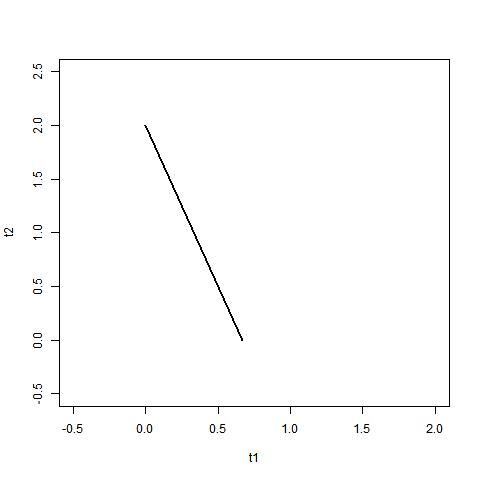
\includegraphics[width=7cm]{graf1.jpg}
\end{center}
\end{frame}
\begin{frame}
\frametitle{Zgled}
Narišemo omejitve: $t_1, t_2 \ge 0$ in $t_1+t_2\le 1$.\pause
\begin{center}
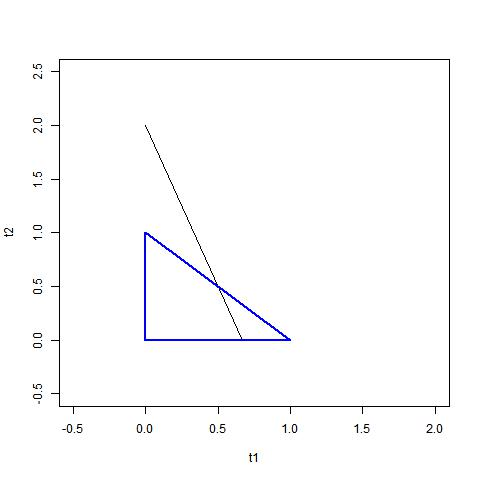
\includegraphics[width=7cm]{graf2.jpg}
\end{center}
\end{frame}
\begin{frame}
\frametitle{Zgled}
Dopustne rešitve za $t_1$ in $t_2$ so dane z daljico v trikotniku.\pause
\begin{center}
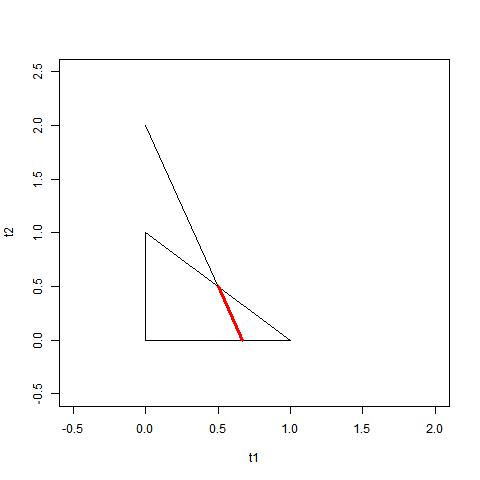
\includegraphics[width=7cm]{graf3.jpg}
\end{center}
\end{frame}
\begin{frame}
\frametitle{Zgled}
Iz daljice lahko izberemo katerikoli par točk $(t_1, t_2)$, npr. $(0.5, 0.5)$. Potem vemo kako izgleda vektor 
$c=\begin{bmatrix}
\sqrt{0.5}\\
\sqrt{0.5}\\
0
\end{bmatrix}$. Iz enačbe $c=X^T b$, dobimo 
$$b=Xc=c =\begin{bmatrix}
\sqrt{0.5}\\
\sqrt{0.5}\\
0
\end{bmatrix}.$$
Seveda je rešitev tudi $b=-c$. Tako dobimo neskončno izotropnih vektorjev $b$.
\end{frame}
\begin{frame}
\frametitle{Neskončno rešitev}
Ta problem za iskanje koeficientov je v treh dimenzijah in možne rešitve $t$-ja so v eni dimenziji. Takšna konstrukcija pripelje do naslednjega izreka:
\begin{izrek}
Če je $n>2$ in $A$ je realna in nedefinitna, ima matrika $H$ vsaj tri različne lastne vrednosti z različnimi predznaki. Potem obstaja neskončno število realnih izotropnih vektorjev.
\end{izrek}\pause
\begin{block}{Splošen zapis}
\begin{equation*}
\sum_{i=1}^{k-1} (\lambda_i -\lambda_k)t_i +\lambda_k =0, \quad t_i\ge0, i=1, \dots,k-1, \sum_{i=1}^{k-1}t_i \le1.
\end{equation*}
\end{block}
\end{frame}
\section{Kompleksne matrike} %KOMPLEKSNE MATRIKE
\subsection{Uvod}
\begin{frame}
\frametitle{Kompleksne matrike}
Predstavljeni bodo algoritmi naslednjih avtorjev:
\begin{enumerate}
\item \emph{Meurant}.
\item \emph{Carden}.
\item \emph{Chorianopoulos, Psarrakos in Uhlig}.
\end{enumerate}
Algoritme bomo numerično primerjali, saj bi radi, da algoritem vrne izotropni vektor s čim manj računanja.
\end{frame}
\subsection{Iskanje izotropnih vektorjev}
\subsubsection{Meurant 1.}
\begin{frame}
\frametitle{Meurant 1.}
\begin{itemize}
\item V nekaterih primerih lahko izračunamo rešitve s samo enim ra\-ču\-na\-njem lastnih vrednosti in vektorjev matrike $K$.
\item Uporabimo lastne vektorje matrike $H$.
\item Z uporabo treh lastnih vektorjev $H$, obstaja neskončno rešitev dobljenih na daljici v trikotniku omejitev.
\item  Če sta imaginarna dela, ki ustrezata robnima točkama daljice, različnih predznakov, potem iz izreka o povprečni vrednosti sledi, da obstaja točka na daljici, ki ima ničeln imaginarni del.
\end{itemize}
\end{frame}
\subsubsection{Meurant 2.}
\begin{frame}
\frametitle{Meurant 2.}
\begin{itemize}
\item Uporabimo lastne vrednosti in lastne vektorje matrike $K=(A-A^\ast)/(2i)$, ki je hermitska. 
\item S kombiniranjem lastnih vektorjev matrike $K$ pripadajočim k pozitivnim in negativnim lastnim vrednostim, lahko (v nekaterih primerih) izračunamo dva vektorja $b_1$ in $b_2$, taka da $$\alpha_1=\Re(b_1^\ast Ab_1)<0$$ in $$\alpha_2=\Re(b_2^\ast Ab_2)>0.$$
\end{itemize}
\end{frame}
%\begin{frame}
%\frametitle{Meurant 2.}
%\begin{lema}\label{komp}
%Naj bosta $b_1$ in $b_2$ enotska vektorja z $\Im(b_i^\ast Ab_i)=0$, $i=1,2$ in $\alpha_1=\Re(b_1^\ast Ab_1)<0, \alpha_2=\Re(b_2^\ast Ab_2)>0$. Naj bo $b(t,\theta)=e^{-i\theta}b_1 + tb_2, t,\theta \in \R, \alpha(\theta)=e^{i\theta}b_1^\ast Ab_2 +e^{-i\theta}b_2^\ast Ab_1.$ Potem je 
%$$b(t,\theta)^\ast Ab(t,\theta)=\alpha_2 t^2 +\alpha(\theta)t+\alpha_1,$$ 
%$\alpha(\theta)\in\R$, ko $\theta=arg(b_2^\ast Ab_1 -b_1^T\bar{A}\bar{b_2}).$ Za $t_1 =(-\alpha(\theta) +\sqrt{\alpha(\theta)^2 -4\alpha_1\alpha_2})/(2\alpha_2)$, imamo 
%$$b(t_1, \theta) \not=0,\quad  \frac{b(t_1,\theta)^\ast}{\norm{b(t_1,\theta)}}A\frac{b(t_1,\theta)}{\norm{b(t_1,\theta)}}=0.$$
%\end{lema}
%\end{frame}
%\begin{frame}
%\frametitle{Meurant 2.}
%\begin{itemize}
%\item  Če imamo $b_1$ in $b_2$, taka da  $\alpha_1=\Re(b_1^\ast Ab_1)<0$ in $\alpha_2=\Re(b_2^\ast Ab_2)>0$, smo končali.
%\item  Ko je $A$ realna in imamo $b_1=x_1, b_2=x_2$ za lastne vektorje $H$, potem je $\theta=0$ in nam lema pove, kako se izračuna en izotropni vektor.
%\item  V kompleksnem primeru, ne moremo vedno najti primerne vektorje $b_1$ in $b_2$.
%\item Ko ne moremo izračunati $b_1$ in $b_2$ potrebnih za lemo, izračunamo lastne vektorje $H$ in uporabimo enako tehniko za matriko $iA$. 
%\item V primeru neuspeha, kombiniramo lastne vektorje $H$ in $K$.
%\end{itemize}
%\end{frame}
%\begin{frame}
%\frametitle{Meurant 2.}
%Naj bo $x$ (oz. $y$) lastna vrednost $K$ (oz. $H$), upoštevamo vektorje $X_\theta =\cos(\theta)x+\sin(\theta)y,$ $0\le\theta\le\pi$. Ko gre $\theta$ od 0 do $\pi$, $X_\theta ^\ast AX_\theta$ opisuje elipso v zalogi vrednosti. Za dan par lastnih vektorjev $x,y$ iščemo presečišča elipse z realno osjo. Opazimo, da je $A=H+iK$, torej imamo:\pause
%\begin{block}{}
%\begin{align*}
%X_\theta^\ast AX_\theta &= \cos^2(\theta)(x^\ast Hx + ix^\ast Kx)\\ 
%&+ \sin^2(\theta)(y^\ast Hy + iy^\ast Ky)\\ 
%&+\sin(\theta)\cos(\theta)(x^\ast Hy +y^\ast Hx +i[x^\ast Ky +y^\ast Kx]).
%\end{align*}
%\end{block}\pause
%Ko enačimo imaginarni del $X_\theta ^\ast AX_\theta$ z 0, dobimo enačbo:\pause
%\begin{block}{}
%$$\alpha \cos^2(\theta) +\beta \sin^2(\theta) +\gamma \sin(\theta)\cos(\theta)=0.$$
%\end{block}
%\end{frame}
%\begin{frame}
%\frametitle{Meurant 2.}
%Naj bo $\alpha=\Im(x^\ast Hx + ix^\ast Kx), \beta=\Im(y^\ast hy +iy^\ast Ky)$ in $\gamma=\Im(x^\ast Hy +y^\ast Hx +i[x^\ast Ky +y^\ast Kx]).$\\ \pause
%Predpostavimo, da $\cos(\theta) \not =0$ in delimo, dobimo kvadratno enačbo za $t=\tan(\theta),$
%\begin{block}{}
%$$\beta t^2 +\gamma t +\alpha =0.$$
%\end{block}
%\begin{itemize}
%\item Če ima ta enačba realne rešitve, potem dobimo vrednosti $\theta$, ki nam vrnejo take vektorje $X_\theta$, da $\Im(X_\theta ^\ast AX_{\theta})=0$. 
%\item Ko je velikost problema velika, ne uporabimo te konstrukcije za vse pare lastnih vektorjev, saj nas to lahko preveč stane. Uporabimo samo lastne vektorje, ki pripadajo par najmanjšim in največjim lastnim vrednostim.
%\item Če tudi ta konstrukcija ne deluje, uporabimo algoritem \emph{Chorianopoulosa, Psarrakosa in Uhliga}.
%\end{itemize}
%\end{frame}
\section{Literatura}
\begin{frame}
\frametitle{Literatura}
\begin{enumerate}
\item
G. Meurant, \emph{The computation of isotropic vectors}, Numer. Alg. {\bf 60} (2012) 193--204.
\item
R. Carden, \emph{A simple algorithm for the inverse field of values problem}, Inverse Probl. {\bf 25} (2009) 1--9
\item
C. Chorianopoulos, P. Psarrakos in F. Uhlig, \emph{A method for the inverse numerical range problem}, Electron. J. Linear Algebra {\bf 20} (2010) 198--206
\item
N. Ciblak, H. Lipkin, \emph{Orthonormal isotropic vector bases}, In: Proceedings of DETC'98, 1998 ASME Design Engineering Technical Conferences (1998).
\item
Johnson, C. R., \emph{Numerical determination of the field of values of a general complex matrix}, SIAM J. Numer. Anal. {\bf15} (1978) 595--602.
\end{enumerate}
\end{frame}
\end{document}

